A valid question is the effect on the limits on each Higgs mass hypothesis in
the case of the presence of a Higgs signal at a given mass. As a test, we
consider a Higgs with $\mHi = 125~\GeV$, and see the effect on the limits, both
cut-based and BDT-based analyses. The expected and observed upper 
limits are reported in Tables~\ref{tab:cutbased_mh125_nj} 
and~\ref{tab:bdtbased_mh125_nj}, and in Figure~\ref{fig:uls_mh125_nj}. 
The observed upper limits in this context are the mean average limits in the presence of background plus signal.

The excess due to the presence of a $\mHi = 125~\GeV$ Higgs is expected to be large in a broad range up to about $\mHi = 160~\GeV$ analysis.
At this mass, both \W\ are on-shell: the kinematic distributions of the Higgs signal change significantly and the shape of the BDT output is clearly 
different (Fig.~\ref{fig:bdt_mh125}).

%%%%%%%%%%%%%%%%%%%%%%%%%%%%%%
\begin{table}[hbp!]
\begin{center}
\begin{tabular}{c c c c c}
\hline
\vspace{-3mm} && \\
 Higgs Mass & Pseudo-data  & Median expected & Expected range for 68\% & Expected range for 95\%   \\
\vspace{-3mm} && \\
\hline
115  & 5.08$\pm$1.11  & 3.02  & [2.18,  4.21]  & [1.62,  5.64] \\
120  & 3.05$\pm$0.62  & 1.77  & [1.28,  2.46]  & [0.95,  3.30] \\
125  & 1.97$\pm$0.40  & 1.18  & [0.85,  1.65]  & [0.63,  2.21] \\
130  & 1.47$\pm$0.24  & 0.84  & [0.61,  1.17]  & [0.45,  1.57] \\
140  & 0.86$\pm$0.16  & 0.51  & [0.37,  0.71]  & [0.27,  0.95] \\
150  & 0.43$\pm$0.09  & 0.32  & [0.23,  0.45]  & [0.17,  0.60] \\
160  & 0.24$\pm$0.04  & 0.20  & [0.14,  0.28]  & [0.11,  0.37] \\
170  & 0.23$\pm$0.04  & 0.20  & [0.15,  0.28]  & [0.11,  0.38] \\
180  & 0.29$\pm$0.06  & 0.26  & [0.19,  0.37]  & [0.14,  0.49] \\
190  & 0.44$\pm$0.09  & 0.39  & [0.28,  0.54]  & [0.21,  0.73] \\
200  & 0.56$\pm$0.11  & 0.48  & [0.35,  0.67]  & [0.26,  0.90] \\
250  & 1.13$\pm$0.25  & 0.97  & [0.70,  1.35]  & [0.52,  1.81] \\
300  & 1.26$\pm$0.26  & 1.12  & [0.81,  1.56]  & [0.60,  2.10] \\
\hline
\end{tabular}
\caption{Upper limits in the 0/1/2-jet bins for SM Higgs using the
  {\bf cut-based} $\mll$ analysis with 5.1$\ifb$ of data in the case of the
  presence of a Higgs with $\mHi = 125~\GeV$.
  The error on the Pseudo-data value corresponds to the standard deviation obtained from 
  100 toy experiments.}
\label{tab:cutbased_mh125_nj}
\end{center}
\end{table}
%%%%%%%%%%%%%%%%%%%%%%%%%%%%%%
%%%%%%%%%%%%%%%%%%%%%%%%%%%%%%
\begin{table}[hbp!]
\begin{center}
\begin{tabular}{c c c c c}
\hline
\vspace{-3mm} && \\
 Higgs Mass & Pseudo-data  & Median expected & Expected range for 68\% & Expected range for 95\%   \\
\vspace{-3mm} && \\
\hline
115  & 4.26$\pm$1.14  & 2.72  & [1.96,  3.78]  & [1.46,  5.07] \\
120  & 2.87$\pm$0.75  & 1.71  & [1.24,  2.39]  & [0.87,  3.19] \\
125  & 1.87$\pm$0.45  & 1.04  & [0.75,  1.44]  & [0.56,  1.93] \\
130  & 1.43$\pm$0.30  & 0.75  & [0.54,  1.04]  & [0.40,  1.39] \\
140  & 0.82$\pm$0.17  & 0.43  & [0.31,  0.60]  & [0.23,  0.80] \\
150  & 0.42$\pm$0.10  & 0.27  & [0.19,  0.37]  & [0.14,  0.50] \\
160  & 0.20$\pm$0.04  & 0.16  & [0.12,  0.23]  & [0.09,  0.31] \\
170  & 0.21$\pm$0.03  & 0.18  & [0.13,  0.25]  & [0.10,  0.33] \\
180  & 0.27$\pm$0.07  & 0.22  & [0.16,  0.31]  & [0.12,  0.42] \\
190  & 0.37$\pm$0.08  & 0.33  & [0.24,  0.46]  & [0.18,  0.62] \\
200  & 0.45$\pm$0.10  & 0.40  & [0.29,  0.56]  & [0.22,  0.75] \\
250  & 0.68$\pm$0.16  & 0.70  & [0.51,  0.98]  & [0.38,  1.31] \\
300  & 0.77$\pm$0.18  & 0.78  & [0.56,  1.08]  & [0.42,  1.45] \\
\hline
\end{tabular}
\caption{Upper limits in the 0/1/2-jet bins for SM Higgs using the
  {\bf shape-based} $\mll$ analysis with 5.1$\ifb$ of data in the case of the
  presence of a Higgs with $\mHi = 125~\GeV$.
  The error on the Pseudo-data value corresponds to the standard deviation obtained from 
  100 toy experiments.}
\label{tab:bdtbased_mh125_nj}
\end{center}
\end{table}
%%%%%%%%%%%%%%%%%%%%%%%%%%%%%%

%%%%%%%%%%%%%%%%%%%%%%%%%%%%%%
\begin{figure}[!hbtp]
\centering
\subfigure[cut-based]{
\centering
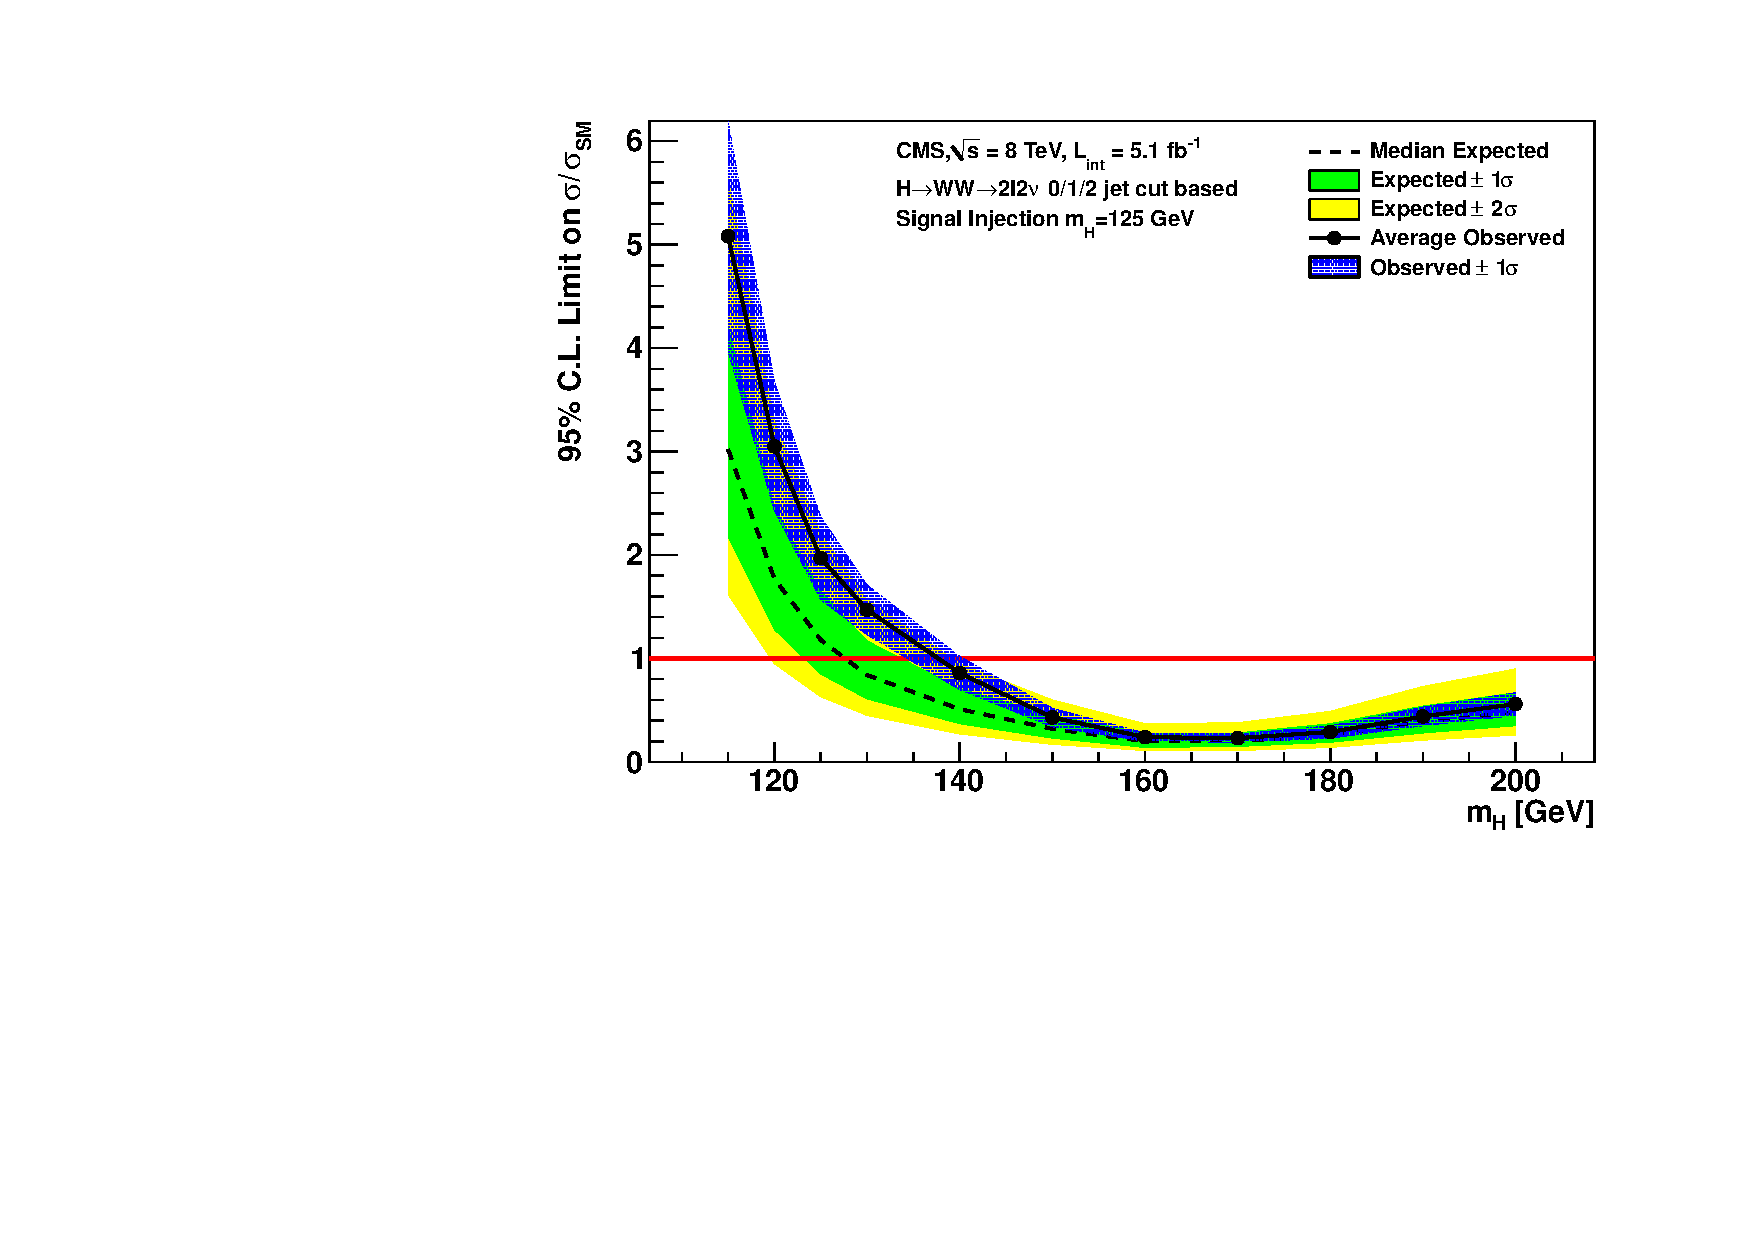
\includegraphics[width=.45\textwidth]{figures/limit_cut_inj125.pdf}
}
\centering
\subfigure[shape-based]{
\centering
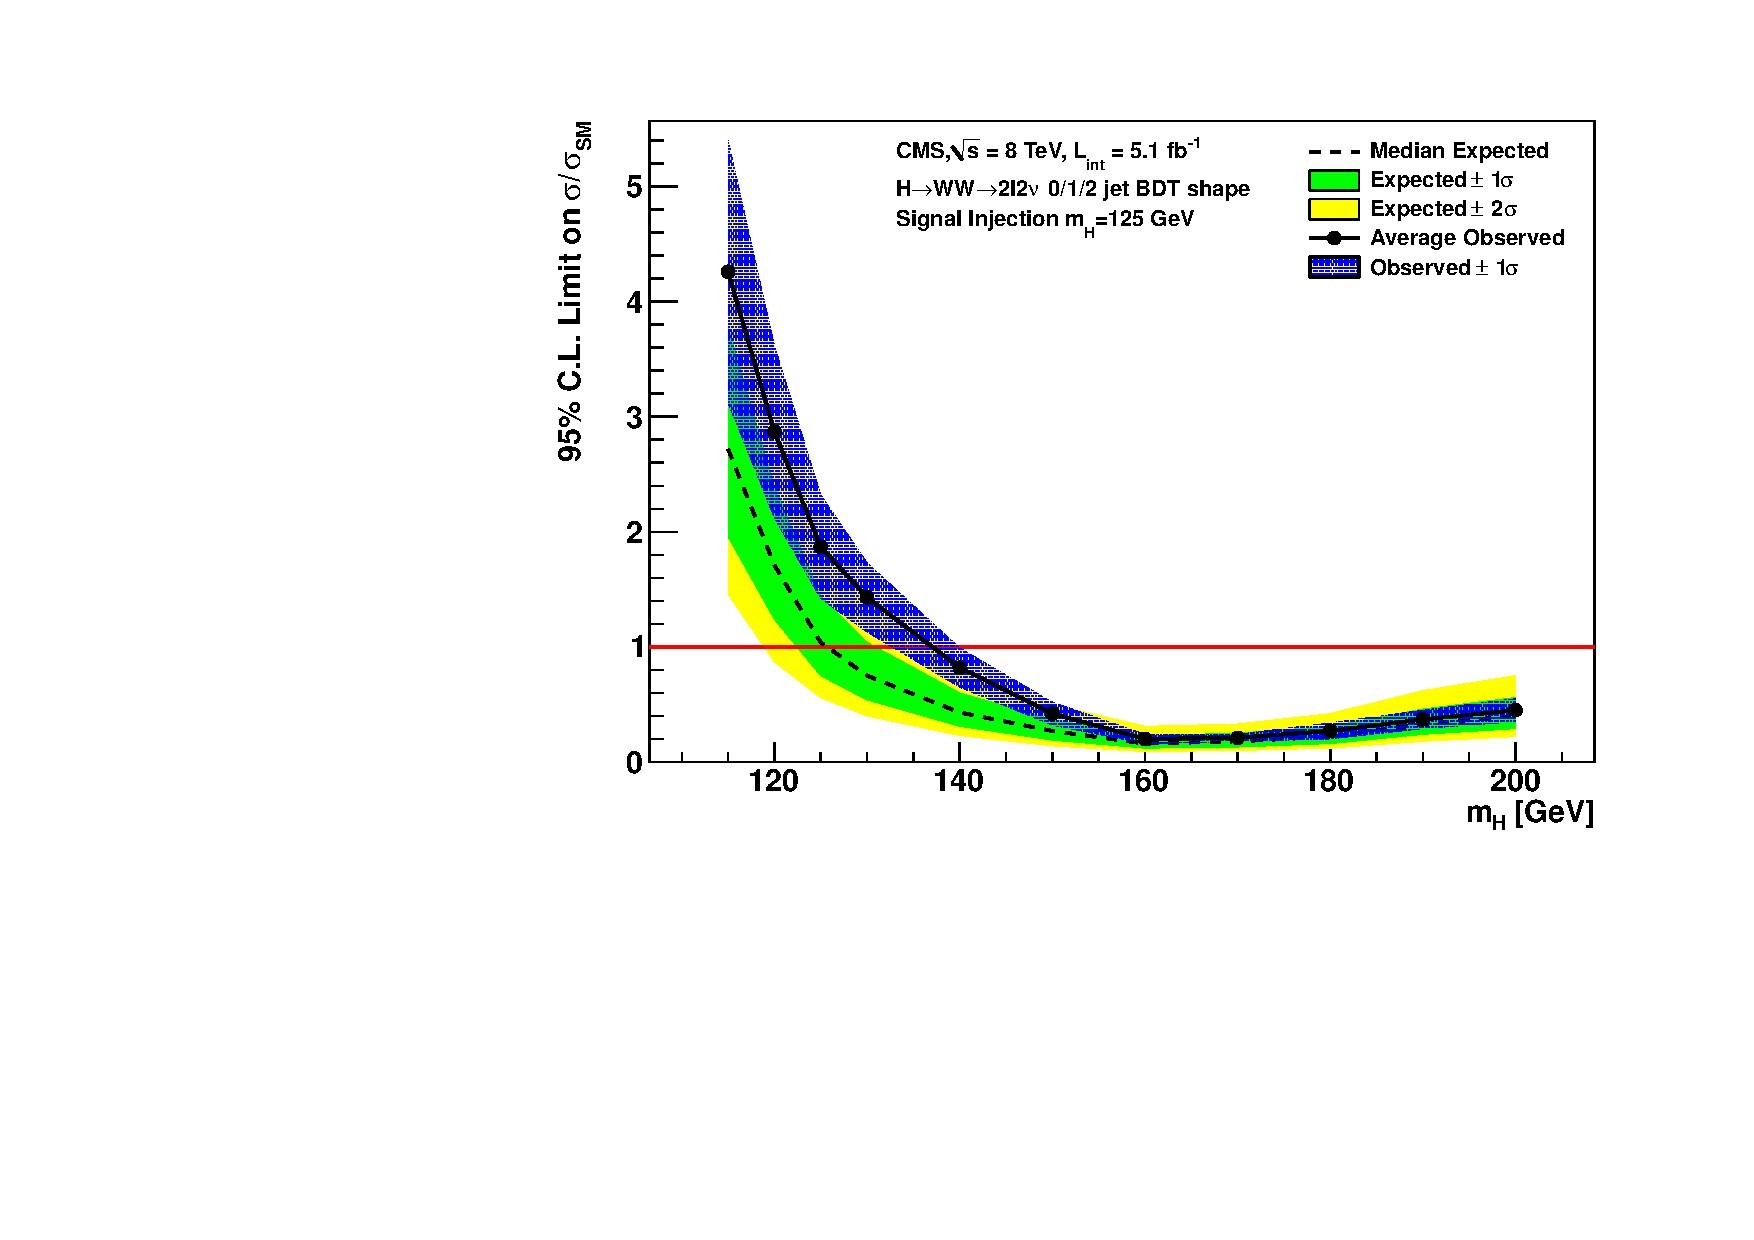
\includegraphics[width=.45\textwidth]{figures/limit_shape_inj125.pdf}
}\\
\subfigure[cut-based (log Y)]{
\centering
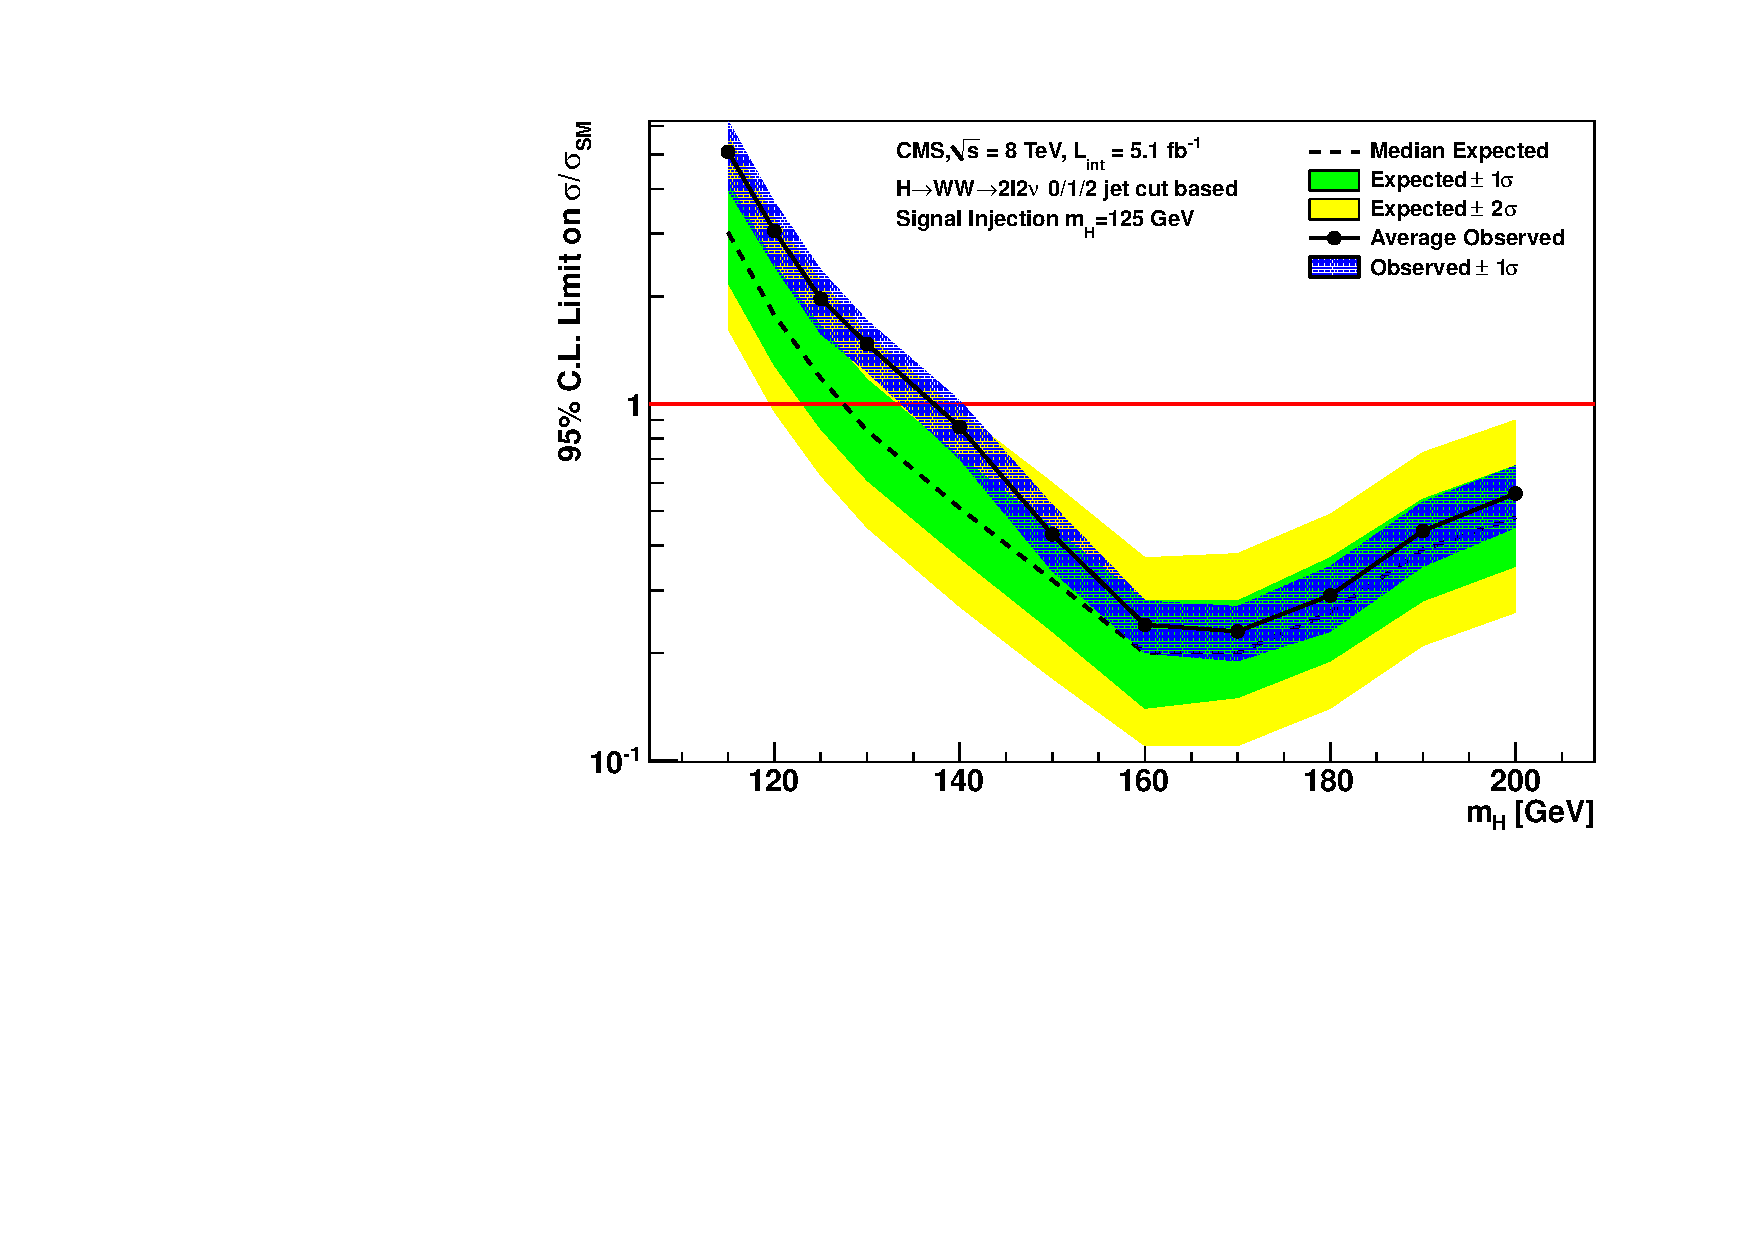
\includegraphics[width=.45\textwidth]{figures/limit_cut_inj125_logy.pdf}
}
\centering
\subfigure[shape-based (log Y)]{
\centering
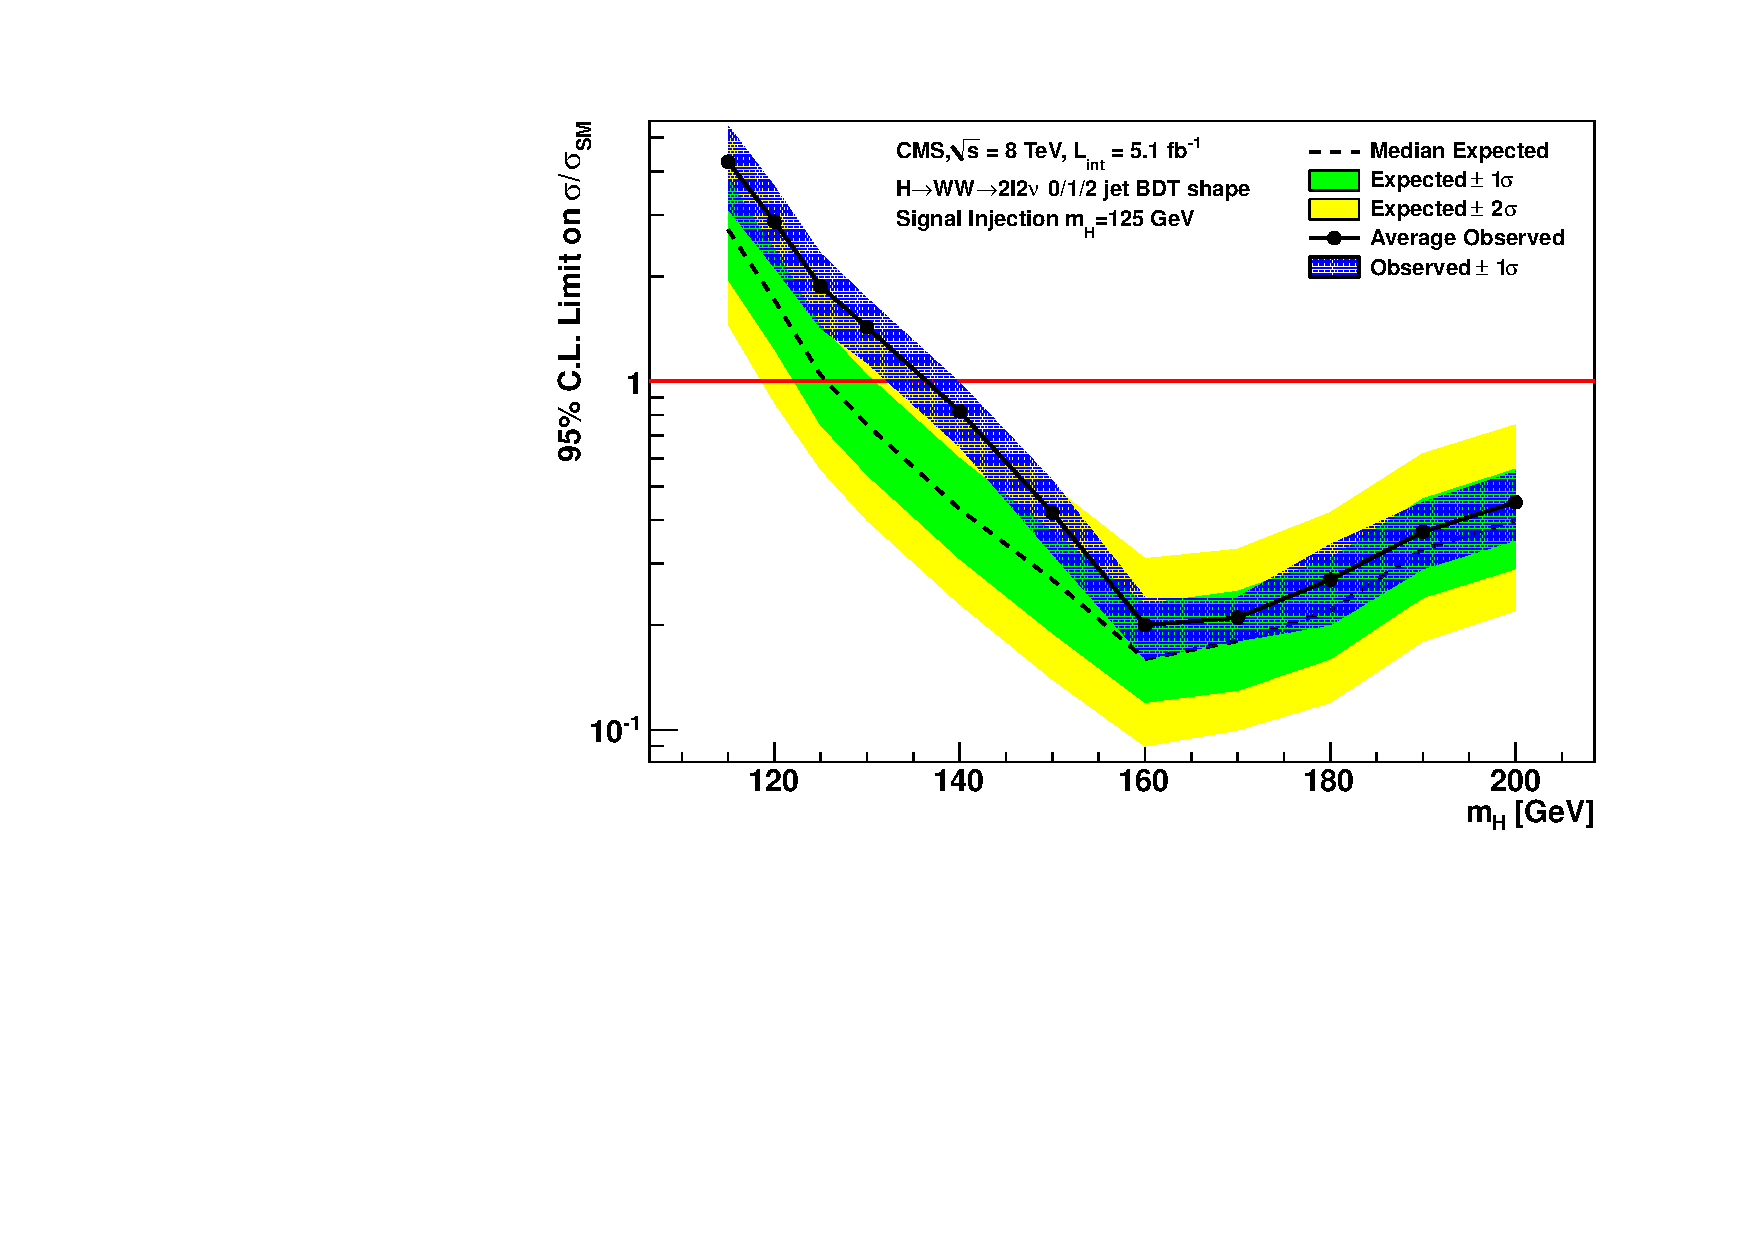
\includegraphics[width=.45\textwidth]{figures/limit_shape_inj125_logy.pdf}
}
\caption{Upper limits in the 0/1/2-jet bins for SM Higgs with 5.1$\ifb$ 
 of data in the case of the presence of a Higgs with $\mHi = 125~\GeV$.
The blue band corresponds to the standard deviation obtained from 
100 toy experiments.}
\label{fig:uls_mh125_nj}
\end{figure}
%%%%%%%%%%%%%%%%%%%%%%%%%%%%%%


%%%%%%%%%%%%%%%%%%%%%%%%%%%%%%
\begin{figure}[!hbtp]
\centering
\subfigure[\mHi=150 \GeVcc\ analysis]{
\centering
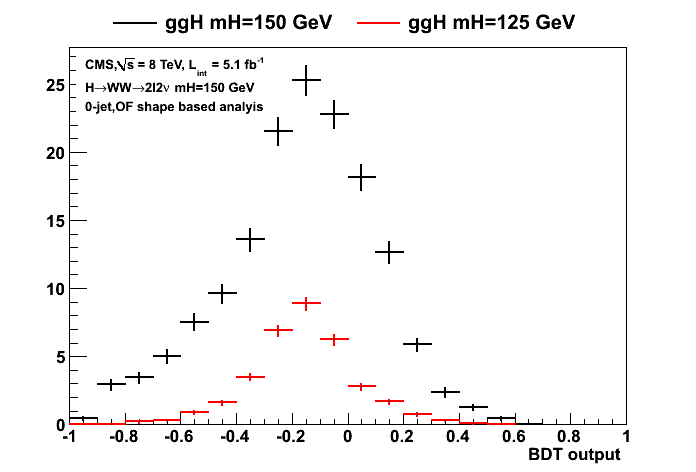
\includegraphics[width=.45\textwidth]{figures/inj125_bdt150.png}
}
\centering
\subfigure[\mHi=160 \GeVcc\ analysis]{
\centering
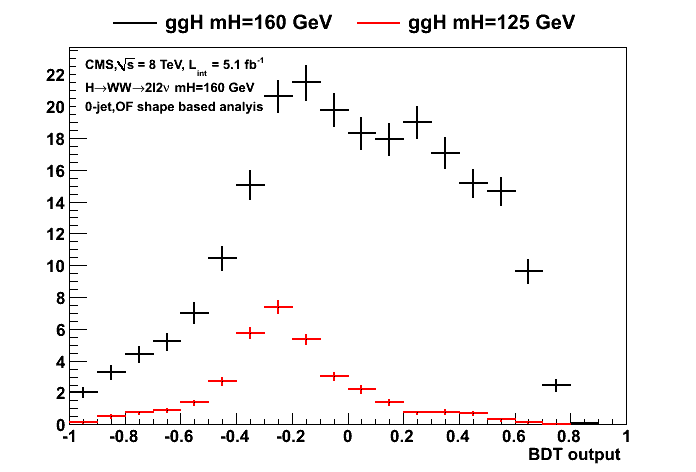
\includegraphics[width=.45\textwidth]{figures/inj125_bdt160.png}
}
\caption{Expected BDT output for a Higgs signal with \mHi=125 and 150 (160) \GeVcc in the 0-jet, OF shape based analysis at  \mHi=150 (160) \GeVcc.}
\label{fig:bdt_mh125}
\end{figure}
%%%%%%%%%%%%%%%%%%%%%%%%%%%%%%
